\documentclass{../cheat}
\title{Statistical Pattern Recognition}
\author{ma.mehralian}
\usepackage{amsmath}

\begin{document}
\begin{multicols}{3}

	\section{1- Introduction}
		\begin{itemize}[nolistsep, leftmargin=1em]
			\item (??) \textbf{Pattern recognition} is the act of taking in raw data and taking an action based on the “category” of the pattern.
			\item (??) \textbf{Pattern classification} is to take in raw data, eliminate noise, and process it to select the most likely model that it represents.
		\end{itemize}
	
		\textbf{Pattern Recognition Approaches}
		\begin{itemize}[nolistsep, leftmargin=1em]
			\item \textbf{Statistical}: Focus on statistics of the patterns.
			\item \textbf{Structural (Syntactic)}: Classifiers are defined using a set of logical rules. Grammars can group rules.
		\end{itemize}
		
		\textbf{Bias-Variance Dilemma}
		\begin{itemize}[nolistsep, leftmargin=1em]
			\item \textbf{Variance}: Simple decision boundaries (e.g., linear) seem to miss some obvious trends in the data.
			\item \textbf{Bias}: Complex decision boundaries seem to lock onto the idiosyncracies of the training data set.
			\item \textbf{Generalization} is the best trade-off.
		\end{itemize}
		\textbf{The Sub-problems of Pattern Classification:}\\ 1-Feature Extraction, 2-Noise, 3-Overfitting, 4-Model Selection, 5-Prior Knowledge, 6-Missing Features, 7-Mereology (the problem of \textit{subsets and supersets}), 8-Segmentation(e.g., in speech recognition), 9-Context(input-dependent information), 10-Invariances (e.g., to translation), 11-Evidence Pooling(e.g., voting), 12-Costs and Risks, 13-Computational Complexity
			
		\subsection{Learning}
		\textbf{Types of Learning}
		\begin{itemize}[nolistsep, leftmargin=1em]
			\item \textbf{Unsupervised learning:	} The system forms clusters or "natural groupings" of the input patterns.
			\item \textbf{Supervised learning:} Classify data using labeled samples.
			\item \textbf{Semi-supervised learning:} make use of both labeled and unlabeled data for training - typically a small amount of labeled data with a large amount of unlabeled data.
			\item \textbf{Reinforcement Learning:} only teaching feedback is available.
		\end{itemize}	
		
		\textbf{Types of Learning (Algorithmic view point)}
		\begin{itemize}[nolistsep, leftmargin=1em]
			\item \textbf{Inductive:} Learns a labeling function over the space
			\item \textbf{Transductive:} Just labels the given test queries
		\end{itemize}	
		
		\textbf{Version Space:}
		Any $h \in H$ between the most specific consistent hypotheses, and the most general consistent hypotheses with training set.

		\textbf{VC Dimension}
		\begin{itemize}[nolistsep, leftmargin=1em]
			\item If a set of examples can be partitioned in all possible ways, we say the hypothesis space $H$ \textbf{shatters} that set of examples.
			\item If we have a set of $N$ examples, we need all possible $2^N$ hypotheses to shatter the set of examples.
			\item VC dimension is the size of the largest finite subset of examples in the input space $X$ shattered  by $H$.
			\item VC dimension can be infinite.
			\item VC dimension of the set of classification functions (H) is: ¨maximum number of training examples (N) that can be shattered  by $H$ or in other word can learned by the machine without error for all possible labeling of the classification functions.
			\item number of points needed to learn a class of interest reliably is proportional to the VC dimension.
			\item In general, the VC dimension of  the space of hyperplanes in $r$ dimensions is $r+1$. 
			\item Suppose that $\text{VC}(H) = d$. Therefore $2d \leq |H|$ and $d = \text{VC}(H) \leq log_2 |H|$.
			\item For a linear classifier VC=d+1 ???????
		\end{itemize}
		
		\textbf{Correctness Criteria:}
		%\setlength{\gapspace}{0.4\columnwidth}
		
		\tab{Precision}$\frac{TP}{TP+FP}$ \\
		\tab{Racal (Hit rate)} 	 $\frac{TP}{TP+FN}$\\
		\tab{Specificity} $\frac{TN}{TN+FP}$ \\
		\tab{Accuracy} $\frac{TP+TN}{TP+TN+FP+FN}$\\
		\tab{Balanced accuracy} $\frac{Racal+Specificity}{2}$\\
		\tab{F-Measure} $2.\frac{Precision.Racal}{Precision+Racal}$
		
%		\begin{tabularx}{\columnwidth}{X X}
%			Precision & $\frac{TP}{TP+FP}$ \\
%			Racal 		& $\frac{TP}{TP+FN}$ \\
%			Specificity & $\frac{TN}{TN+FP}$ \\
%			Accuracy 		& $\frac{TP+TN}{TP+TN+FP+FN}$ \\
%			Balanced accuracy & $\frac{Racal+Specificity}{2}$ \\
%			F-Measure 		& $2.\frac{Precision.Racal}{Precision+Racal}$ \\
%		\end{tabularx}
	
	
	\section{2- Bayesian decision theory}	
	\textbf{Bayes' formula:}

	\tab{$P(\omega_j|x) = \frac{p(x|\omega_j)P(\omega_j)}{p(x)}$}
		$posterior = \frac{likelihood \times prior}{evidence}$
	
	\textbf{Bayes' decision rule:}
	\[ \begin{array}{cc}
		P(\omega_1|x) \operatorname*{\lessgtr}_{\omega_1}^{\omega_2} P(\omega_2|x) \quad \null & \null \quad
		\omega^* = \operatorname*{arg\,max}_{i} P(\omega_i|x)
	\end{array}\]
	\begin{itemize}[nolistsep, leftmargin=1em]
		\item Under this rule $P(error|x) = \min [P(\omega_1|x), P(\omega_2|x)]$.
		\item By eliminating this scale factor $p(x)$: 
		\[P(x|\omega_1) P(\omega_1) \operatorname*{\lessgtr}_{\omega_1}^{\omega_2} P(\omega_2|x) P(\omega_2)\]
	\end{itemize}
	
	\subsection{Bayesian Decision Theory}
	\textbf{Loss Function}
	\begin{itemize}[nolistsep, leftmargin=1em]
		\item The loss function states exactly how costly each action is, and is used to convert a probability determination into a decision.
		\item The loss function $\lambda_{ij}=\lambda(\alpha_i|\omega_j)$ describes the loss incurred for taking action $\alpha_i$ when the state of nature (class) is $\omega_j$.
	\end{itemize}
	
	\textbf{Risk}
	\begin{itemize}[nolistsep, leftmargin=1em]
		\item An expected loss is called a risk.\\
			\centerline{$R(\alpha_i|\mathrm{x}) =\sum_{j=1}^c \lambda(\alpha_i|\omega_j) P(\omega_j|\mathrm{x})$.}
		\item $R(\alpha_i|\mathrm{x})$ is the conditional risk associated with action $\alpha_i$.
		\item The overall risk is the expected loss associated with a given decision rule. $ R =\int R(\alpha(\mathrm{x})|\mathrm{x}) p(\mathrm{x}) d\mathrm{x}$
		\item minimum-risk decision rule: $\omega_1$ if $R(\alpha_1|\mathrm{x}) < R(\alpha_2|\mathrm{x})$ where \\
			\centerline{$R(\alpha_1|\mathrm{x}) = \lambda_{11}P(\omega_1|\mathrm{x}) + \lambda_{12}P(\omega_2|\mathrm{x})$}\\
			\centerline{$R(\alpha_2|\mathrm{x}) = \lambda_{21}P(\omega_1|\mathrm{x}) + \lambda_{22}P(\omega_2|\mathrm{x})$}\\
		SO: $\begin{array}{r c l}
			(\lambda_{21}-\lambda_{11}) P(\omega_1|\mathrm{x}) &>& (\lambda_{12}-\lambda_{22}) P(\omega_2|\mathrm{x})\\
			(\lambda_{21}-\lambda_{11}) p(\mathrm{x}|\omega_1) P(\omega_1) &>& (\lambda_{12}-\lambda_{22}) p(\mathrm{x}|\omega_2) P(\omega_2)
		\end{array}  $\\
		likelihood ratio $\frac{p(\mathrm{x}|\omega_1)}{p(\mathrm{x}|\omega_2)} > \frac{\lambda_{12}-\lambda_{22}}{\lambda_{21}-\lambda_{11}} \frac{P(\omega_2)}{P(\omega_1)}$
	\end{itemize}

	\subsection{Minimum-Error-Rate Classification}
	\begin{itemize}[nolistsep, leftmargin=1em]
		\item \textit{symmetrical} or \textit{zero-one} loss function\\ 
			\centerline{ $\lambda_{ij}= \left\{ \begin{array}{rc}
				0 & i=j\\
				1 & i \neq j
			\end{array}\right.$}\\
			$R(\alpha_i|\mathrm{x}) = 1-P(\omega_i|\mathrm{x}) $
	\end{itemize}
	
	\textbf{Minimax Criterion}
	\begin{itemize}[nolistsep, leftmargin=1em]
		\item minimize the maximum possible overall risk.
		\item minimax risk: $\begin{array}{ll}
		 R_{mm} &= \lambda_{22}+(\lambda_{12}-\lambda_{22})\int_{\mathcal{R}_1} p(\mathrm{x}|\omega_2) d \mathrm{x}\\
		 &= \lambda_{11}+(\lambda_{21}-\lambda_{11})\int_{\mathcal{R}_2} p(\mathrm{x}|\omega_1) d \mathrm{x}
		\end{array}$
	\end{itemize}
	
	\textbf{Neyman-Pearson Criterion}: minimize the overall risk subject to a constraint.
	
	
	2.4 Classifiers, Discriminant Functions????????????
	
	
	\subsection{The Normal Density}
	\textbf{Univariate Density}:
	$p(x) = \frac{1}{{\sigma \sqrt {2\pi } }}e^{{{ - \left( {x - \mu } \right)^2 } \mathord{\left/
	 {\vphantom {{ - \left( {x - \mu } \right)^2 } {2\sigma ^2 }}} \right.
	 \kern-\nulldelimiterspace} {2\sigma ^2 }}}$\\
	\centerline{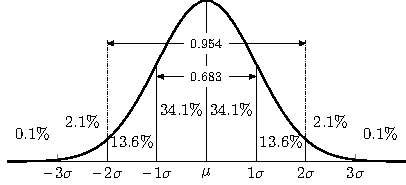
\includegraphics[scale=.8]{plots/gaussian_2d}}

	\textbf{Entropy}
	\begin{itemize}[nolistsep, leftmargin=1em]
		\item The entropy is a non-negative quantity that describes the fundamental uncertainty in the values of points selected randomly from a distribution.\\
			\centerline{$H(p(x)) = - \int {p(x) \ln p(x)dx}$}
		\item measured in \textit{nats}. If a $\log_2$ is used instead, the unit is the \textit{bit}.
		\item The uniform distribution has maximum entropy (on a given interval).
		\item Normal distribution has the maximum entropy of all distributions having a given mean and variance
		\item \textbf{Central Limit Theorem}: The aggregate effect of a large number of small, independent random disturbances will lead to a Gaussian distribution
	\end{itemize}
	
	\textbf{Multivariate Density:}\\
	\centerline{$N(\mu, \Sigma)=P(\mathtt{x})=\frac{1}{(2\pi)^{d/2}\vert\Sigma\vert^{1/2}}e^{-\frac{1}{2}(\mathrm{x}-\mu)^t\Sigma^{-1}(\mathrm{x}-\mu)}$}
	%\\ \centerline{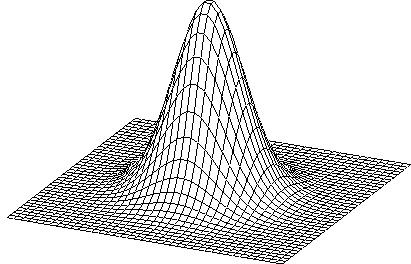
\includegraphics[scale=.6]{plots/gaussian_3d}}

	\begin{itemize}[nolistsep, leftmargin=1em]
		\item For $p(\mathrm{x}) \sim N(\mu,\Sigma)$ and $A_{d\times k}$, define $\mathrm{y} = A^t x$ then:\\
			\centerline{ $p(\mathrm{y}) \sim N(A^t\mu,A^t \Sigma A)$}
		\item \textbf{Whitening transformation}: If we define $\Phi$ to be the matrix whose columns are the orthonormal eigenvectors of $\Sigma$, and $\Lambda$ the diagonal matrix of the corresponding eigenvalues, then the transformation $A_w = \Phi\Lambda^{-1/2}$ applied to the coordinates insures that the transformed distribution has covariance matrix equal to the identity matrix.
	The transform $A_w$ is called a \textit{whitening transformation}.	
		\item \textbf{Mahalanobis distance:} $r^2=(\mathrm{x}-\mu)^t\Sigma^{-1}(\mathrm{x}-\mu)$
	\end{itemize}
	
	\textbf{Missing Features:}
	\begin{itemize}[nolistsep, leftmargin=1em]
		\item let $\mathrm{x} = [\mathrm{x}_g, \mathrm{x}_b]$, where $x_g$ represents the known or "good" features and $\mathrm{x}_b$ represents the "bad" ones.
		\item $P(\omega_j|\mathrm{x}_g)=\frac{\int P(\omega_i,\mathrm{x}_g,\mathrm{x}_b) d\mathrm{x}_b}{p(\mathrm{x}_g)}=\frac{\int P(\omega_i|\mathrm{x}_g,\mathrm{x}_b) p(\mathrm{x}_b,\mathrm{x}_g) d\mathrm{x}_b}{p(\mathrm{x}_g)}$
		\item we must integrate (marginalize) the posterior probability over the bad features. Finally we
use the Bayes decision rule on the resulting posterior probabilities, i.e., choose $\omega_i$ if $P(\omega_i|\mathrm{x}_g) > P(\omega_j |\mathrm{x}_g)$ for all $i$ and $j$.
	\end{itemize}
	

	\section{3-ML and Bayesian parameter estimation}
		\textbf{parameter estimation}
		\begin{itemize}[nolistsep, leftmargin=1em]
			\item \textbf{Maximum Likelihood (ML):} Maximum likelihood and several other methods view
the parameters as quantities whose values are fixed but unknown. The best estimate
of their value is defined to be the one that maximizes the probability of obtaining
the samples actually observed.
			\item \textbf{Bayesian:} Bayesian methods view the parameters as
random variables having some known a priori distribution.
		\end{itemize}
	
		\subsection{Maximum Likelihood Estimation}
		\begin{itemize}[nolistsep, leftmargin=1em]
			\item Nearly always have good convergence properties as the number of training samples increases. 
			\item	Maximum likelihood estimation often can be simpler than alternate methods, such as Bayesian techniques.
			\item Our problem is to use the information provided by the training samples to obtain good estimates for the unknown parameter vectors $\theta_1, ... , \theta_c$ associated with each category.
			\item $\mathcal{D}$ is the set of \textbf{i.i.d} training samples and $\theta$ is unknown parameters. So,  $p(\mathcal{D}|\theta)=\prod_{k=1}^{n} p(x_k|\theta)$.
		\end{itemize}
	
		\textbf{log-likelihood}
		\begin{itemize}[nolistsep, leftmargin=1em]
			\item We define $l(\theta)$ as the log-likelihood function:\\
				\centerline{$l(\theta) \equiv \text{ln} \; p(\mathcal{D}|\theta) =\sum_{k=1}^{n} \text{ln} \; p(\mathrm{x}_k|\theta)$}
		 	\item $\hat{\theta}$ is estimated parameters and $\hat{\theta}=\theta$ when $n \rightarrow \infty$
		 		\[\hat{\theta}=\operatorname*{arg\,max}_\theta l(\theta)\]
		 	\item Let $\Delta_\theta$ be the gradient operator, then\\
		 		\centerline{$\Delta_\theta l(\theta)=\sum_{k=1}^{n} \Delta_\theta \text{ln} \; p(x_k|\theta)$}
		 	\item Thus, a set of necessary conditions for the ML estimate for $\theta$ can be
obtained from the set of $p$ equations:\\
				\centerline{$\Delta_\theta l=0$}
		\end{itemize}
	
		\textbf{Gaussian Case}
		\begin{itemize}[nolistsep, leftmargin=1em]
		 	\item Sample mean ($\hat{\mu}_n$): $\frac{1}{n} \sum_{k=1}^n \mathrm{x}_k$
		 	\item Sample variance ($\widehat{\Sigma}_n$): 
		 		$\frac{1}{n} \sum_{k=1}^n (\mathrm{x}_k-\hat{\mu}) (\mathrm{x}_k-\hat{\mu}) ^t$\\
		 	 - The maximum likelihood estimate for the variance is biased.
		\end{itemize}
		
		
		\subsection{Bayesian estimation}
			\begin{itemize}[nolistsep, leftmargin=1em]
				\item In Bayesian learning we consider $\theta$ to be a random variable, and training data allows us to convert a distribution on this variable into a posterior probability density.
				\item The primary task in Bayesian Parameter Estimation is the computation of the posterior density $p(\theta|D)$ by Bayes formula.
			\end{itemize}
	
			\textbf{The Class-Conditional Densities}
			\begin{itemize}[nolistsep, leftmargin=1em]
				\item Given the sample $\mathcal{D}$, Bayes’ formula then becomes:\\
					\centerline{$P(\omega_i|\mathrm{x},D) = \frac{p(\mathrm{x}|\omega_i,\mathcal{D})P(\omega_i|\mathcal{D})}{\sum^c_{j=1} p(\mathrm{x}|\omega_j ,\mathcal{D}) P(\omega_j|\mathcal{D})}$}
				
				\item with the samples in $\mathcal{D}_i$ belonging to $\omega_i$:\\
					\centerline{$P(\omega_i|\mathrm{x},D) = \frac{p(\mathrm{x}|\omega_i,\mathcal{D}_i)P(\omega_i)}{\sum^c_{j=1} p(\mathrm{x}|\omega_j ,\mathcal{D}_j) P(\omega_j)}$}
			\end{itemize}
			
			\textbf{Parameter Distribution:}\\
			\centerline{$p(\mathrm{x}|\mathcal{D}) = \int p(\mathrm{x}, \theta | \mathcal{D}) d\theta = \int p(\mathrm{x}| \theta) p(\theta | \mathcal{D}) d\theta$}
			
		\subsection{Recursive Bayesian Estimation}
			???	
	--
		
			\textbf{When do ML and Bayes methods differ?}
			\begin{itemize}
				\item ML and Bayes solutions are equivalent in the
asymptotic limit of infinite training data.
				\item ML methods are often to be prefered computationally.
				\item ML: require merely differential calculus techniques or gradient search for $\hat{\theta}$
				\item Baysian: need complex multidimensional integration.
				\item ML: easier to interpret and understand.
				\item Bayesian methods use more of the information brought to the problem than do ML methods. If such information is reliable, Bayes methods can be expected to give better results.
			\end{itemize}	


	\section{4-Nonparametric Methods}
		\begin{itemize}
			\item Most real-world entities have multimodal distributions whereas all classical parametric densities are unimodal.
			\item \textbf{nonparametric}: arbitrary distributions and without the assumption that the underlying form of the densities are known. e.g., Histograms, Kernel Density Estimation/Parzen Windows, k-Nearest Neighbor Density Estimation.
		\end{itemize}
		
		
		\textbf{Histogram Density Estimator}
		\begin{itemize}
			\item \textbf{Advantages:}
				\begin{itemize}
					\item Simple to evaluate and simple to use.
					\item One can throw away $\mathcal{D}$ once the histogram is computed.
					\item Can be computed sequentially if data continues to come in.
				\end{itemize}
			\item \textbf{Disadvantages:}
				\begin{itemize}
					\item The estimated density has discontinuities due to the bin edges rather than any property of the underlying density.
					\item Scales poorly (curse of dimensionality): we would have $M^D$ bins if we divided each variable in a $D$-dimensional space into $M$ bins.
				\end{itemize}
		\end{itemize}
		
		\textbf{Density estimation}
		\begin{itemize}
			\item Let $\mathcal{R}$ denote a small region containing $\mathrm{x}$.
			\item The probability $P$ that a vector $\mathrm{x}$ will fall in a region $\mathcal{R}$ is given by $P=\int_\mathcal{R} p(\mathrm{x}')d\mathrm{x}'$
			\item The probability that $k$ of these $n$ samples fall in $\mathcal{R}$ is given by the binomial law $P_k=\left( \begin{array}{c} n \\ k \end{array} \right)p^k (1-p)^{n-k}$
			\item and the expected value for k is $E[K]=nP$
			\item Assuming continuous $p(x)$ and that $\mathcal{R}$ is so small that $p(x)$ does not appreciably vary within it, we can write:
				$\int_\mathcal{R} p(x')dx' \simeq p(x)V$
				where $x$ is a point within $\mathcal{R}$ and $V$ is the volume enclosed by $\mathcal{R}$.
				SO: $p(x) \simeq \frac{k}{nV}$
			\item SO what ... ????
			\item ...
			\item ...
			\item There are two common ways of obtaining regions that satisfy these conditions:
				\begin{itemize}
					\item Shrink an initial region by specifying the volume $V_n$ as some function of n such as $V_n = 1/\sqrt{n}$. Then, we need to show that $p_n(\mathrm{x})$ converges to $p(\mathrm{x})$. (e.g, Parzen window)
					\item Specify $k_n$ as some function of n such as $V_n = 1/\sqrt{n}$. Then, we grow the volume $V_n$ until it encloses $k_n$ neighbors of $\mathrm{x}$. (e.g., k-nearest-neighbor).
				\end{itemize}
		\end{itemize}
		
		
		\textbf{Parzen windows}
		\begin{itemize}
			\item assuming that the region $\mathcal{R}_n$ is a d-dimensional hypercube.
			\item $k_n$: The number of samples falling in the hypercube, by defining window function $\varphi(u)$
		\end{itemize}

		\textbf{$k_n$ Nearest Neighbor Methods}
		\begin{itemize}
			\item Selecting the best window/bandwidth is a severe limiting factor for Parzen window estimators.
			\item $k_n$-NN methods circumvent this problem by making the window size a function of the actual training data.
			\item The basic idea here is to center our window around $\mathrm{x}$ and let it grow until it capture $k_n$ samples
		\end{itemize}
		
		\section{5-Linear Discriminant Functions}
		\subsection{Linear Discriminant Function}
		\textbf{The Two-Category Case:}\
		\begin{itemize}
			\item Discriminant function: $g(\mathrm{x}) = \mathrm{w}^t \mathrm{x} + w_0$\\
				where $\mathrm{w}$ is the weight vector and $w_0$ the bias or threshold weight.
			
			\item The distance from $\mathrm{x}$ to the hyperplane.\\
				\centerline{$\mathrm{x} = \mathrm{x}_p + r \frac{\mathrm{w}}{\Vert \mathrm{w} \Vert}; \quad r = \frac{g(\mathrm{x})}{\Vert w\Vert}$}
				where $\mathrm{x}_p$ is the normal projection of $\mathrm{x}$ onto $H$, and $r$ is the desired algebraic distance.
				positive if $\mathrm{x}$ is on the positive side and negative if $\mathrm{x}$ is on the negative side.
		\end{itemize}
		
		
		\textbf{The Multi-Category Case:}
		\begin{itemize}
			\item reduce the problem to $c - 1$ two-class problems
			\item use $c(c-1)/2$ linear discriminants, one for everypair of classes.
		\end{itemize}

		
		
		\subsection{Generalized Linear Discriminant Functions}
		\begin{itemize}
			\item Linear discriminant function: $g(x) = w_0 + \sum_{i=1}^{d} w_i x_i$
			\item Quadratic discriminant function:\\
				\centerline{$g(x) = w_0 + \sum_{i=1}^{d} w_i x_i + \sum_{i=1}^{d} \sum_{j=1}^{d} w_{ij} x_i x_j$}
			\item Generalized linear discriminant function:\\
				\centerline{$g(x) =  \sum_{i=1}^{\hat{d}} a_i y_i(x)=\mathrm{a}^t \mathrm{y}$}\\
				$\mathbf{y}$ augmented feature vector, $\mathbf{a}$ augmented weight vector
			\item The $\hat{d}$ functions $y_i(x)$ merely map points in $d$-dimenional $\mathrm{x}$-space to points in $\hat{d}$-dimensional $\mathrm{y}$-space.
			\item The resulting discriminant function is not linear in $\mathrm{x}$, but it is linear in $\mathrm{y}$.
			\item The hyperplane decision surface $\hat{H}$ defined by $\mathrm{a}^t \mathrm{y}=0$
			
		\end{itemize}
		
		
		\subsection{The Two-Category Linearly-Separable Case}
		\begin{itemize}
			\item if exists a weight vector that classifies all of the samples correctly, the samples are said to be \textbf{linearly separable}.
		\end{itemize}
	
% You can even have references
\vspace{5mm}
\rule{0.3\linewidth}{0.25pt}
\scriptsize

\textbf{References:}
\begin{itemize}[leftmargin=2em]
	\item [{[1]}] Pattern Classification, by Richard O. Duda, David G. Stork, Peter E. Hart
\end{itemize}
Made by \href{http://webpages.iust.ac.ir/mehralian/}{ma.mehralian} using \LaTeX
\end{multicols}

\end{document}